\documentclass{article}
 
\usepackage{cite}
\usepackage{graphicx}
\usepackage{wrapfig}
\usepackage[final]{pdfpages}

\graphicspath{{figures/}}
\renewcommand{\code}{\texttt}

\begin{document}
\section{Distribution overview}
The code distribution contains two top level directories. \code{docs} and \code{src}. Additionally, there may be miscellaneous files such as \code{readme.md}, \code{license.txt}, and \code{.gitignore}} at the top level.

\code{docs} contains documentation, both source .tex and output .pdf files.

\code{src} contains the source and ancillary files for all of the microservices that make up the BDA Service. These services are show graphically in Figure~\ref{fig:flowchart}. Additionally, there are directories within \code{src} that contain scripts to deploy the BDA Service.
\begin{figure}
\centering
\includegraphics[width=0.9\textwidth]{figures/bda_flowchart.png}
\caption{\label{fig:flowchart}Overview of the BDA Service Architecture}
\end{figure}

\section{Deployment}
\subsection{Dockerizing BDA Service}
The distribution includes scripts for creating all the microservice docker images to instantiate the BDA Service either locally or in the cloud. The intent is to deploy the Service to a kubernetes cluster.

The main script to create the needed docker images is \code{src/docker/build\_images.sh}. This script can be from the \code{src} directory. Before running this script, it is important to do two things: First, edit the script variable \code{roottag} to point to a docker registry that will be used for deployment to the cloud. This may be an AWS, Azure, or other registry. A local registry can be used if you plan to run the Service locally or to manually push images to the cloud registry. Second, make sure the current user has authenticated to the registry.  Useful flags during building are include the following:

\code{-p } build and then push to the registry

\code{-R [registry name]} update default registry name before building.

Running this script should incorporate all the code into docker images and optionally push this image to where a cluster will pick them up, create containers from them, and run them as the BDA Service.

\subsection{Kubernetes}
The intent of this code is to send it into the kubernetes (k8s) cluster in the cloud for efficient use of powerful resources. Basic scripts needed to do this are in the \code{src/k8s} directory, although a knowledgeable user of k8s will likely wish to make changes to this deployments.

The \code{Cluster\_start.sh} script creates and uses a set of k8s yaml files in a directory structure based on the image registry in which the docker images reside. For instance, if the images were pushed to \code{reg.aws.io/myReg}, then \code{Cluster\_start.sh}} will create a series of k8s yaml files in \code{k8s/reg.aws.io/myReg/} with image specifications inside those files pointing to \code{reg.aws.io/myReg}. This behavior is directed by the \code{-R [registry name]} flag to \code{Cluster\_start.sh}. 

The \code{Cluster\_start.sh} script also does a \code{kubectl apply -f} to these files, one at a time (or a \code{kubectl delete -f} if the \code{-d} flag is specified) to start up (or shut down) the various containers and services.

\begin{figure}
\centering
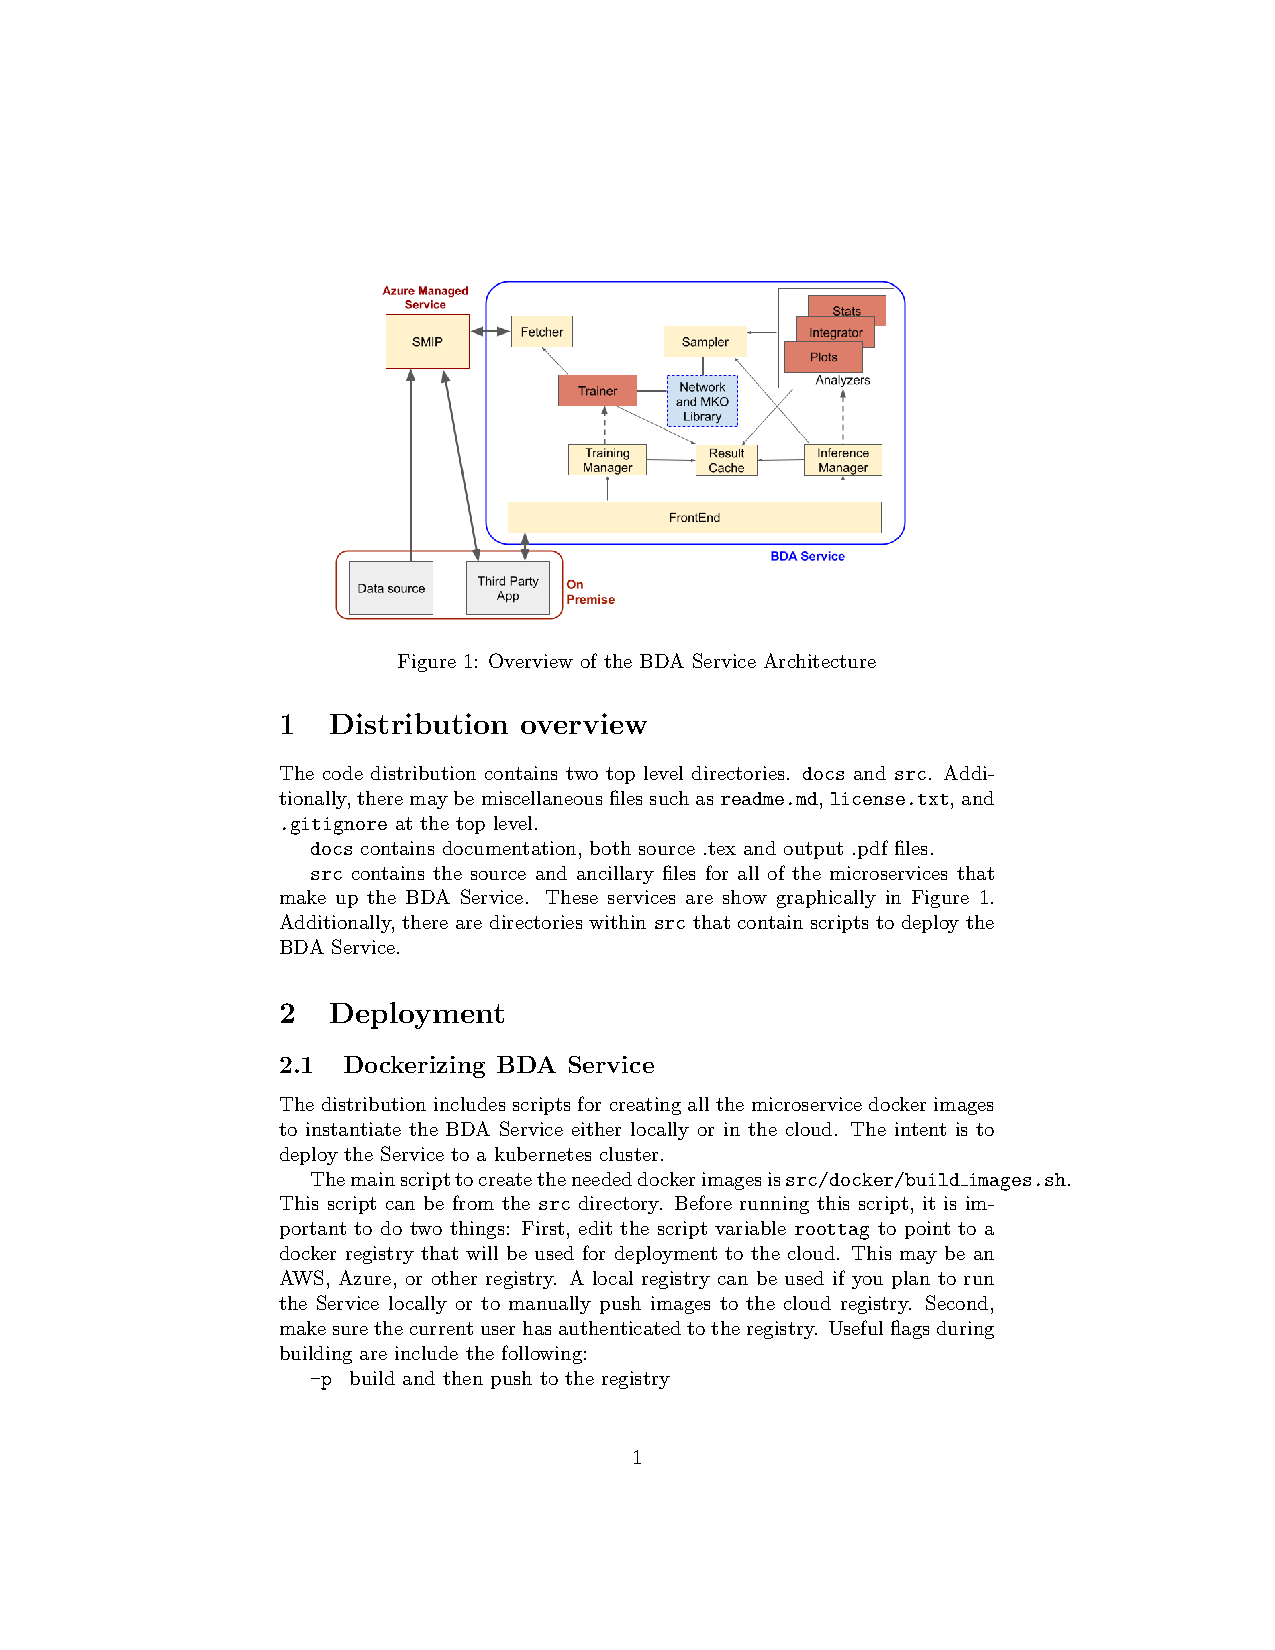
\includegraphics[width=0.9\textwidth]{figures/deployment.png}
\caption{\label{fig:deployment}kubectl view of deployed BDA service, including external access IP address (here 20.141.182.107:5000)}
\end{figure}

The \code{frontend-service} service acts as an ingress point into the k8s cluster on port 5000. The external IP address for this ingress point can be seen (as in Figure~\ref{fig:deployment} by using \code{kubectl get service} or \code{kubectl get all}. 